\documentclass[10pt]{article} 
\usepackage{simpleConference}
\usepackage[utf8]{inputenc}
\usepackage{times}
\usepackage{graphicx}
\usepackage{amsmath, amsthm, amssymb}

% additional packages
\usepackage{tikz, tikz-3dplot} 
\usetikzlibrary{calc}
\usepackage{bbm}
\usepackage{support-caption}
\usepackage{subcaption}
\usetikzlibrary{matrix}
\usepackage{url}
\usepackage{float}
 
\begin{document}
\pagenumbering{gobble}

\begin{figure}[H]
\centering
\begin{subfigure}{.25\textwidth}
  \centering
  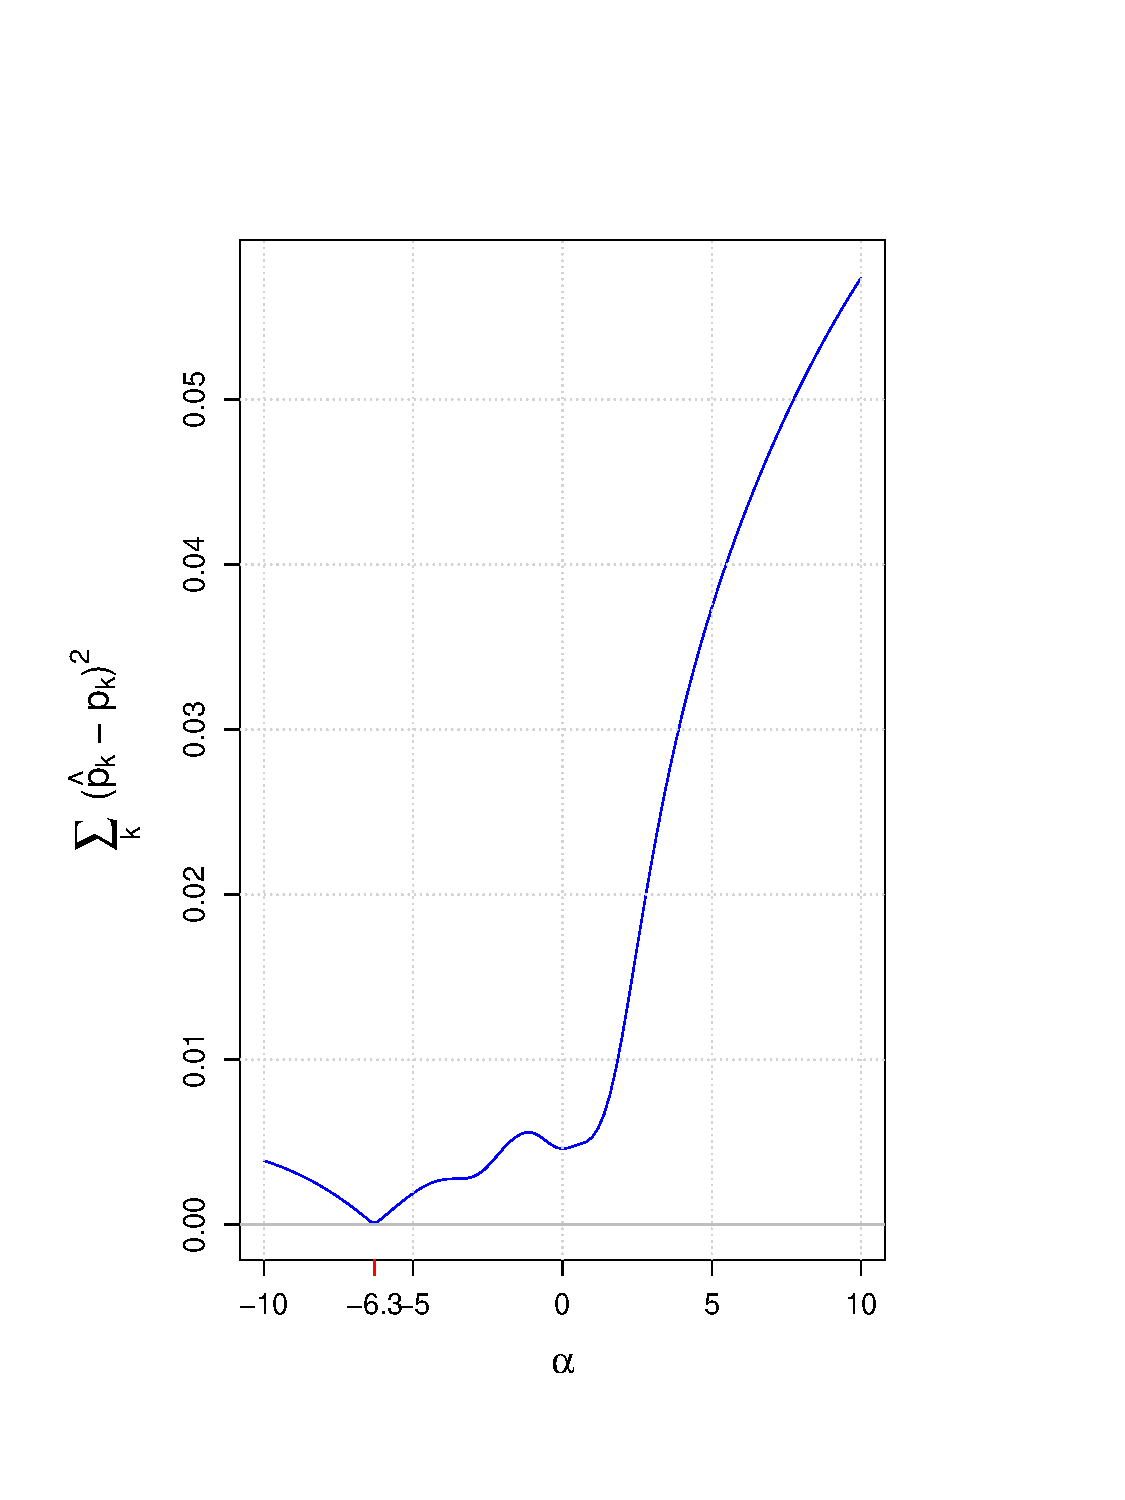
\includegraphics[width=\linewidth]{alpha_trace_-6_3.pdf}
  \caption{ $\alpha = -6.3$.}
  \label{fig: alpha_negative}
\end{subfigure}%
\begin{subfigure}{.25\textwidth}
  \centering
  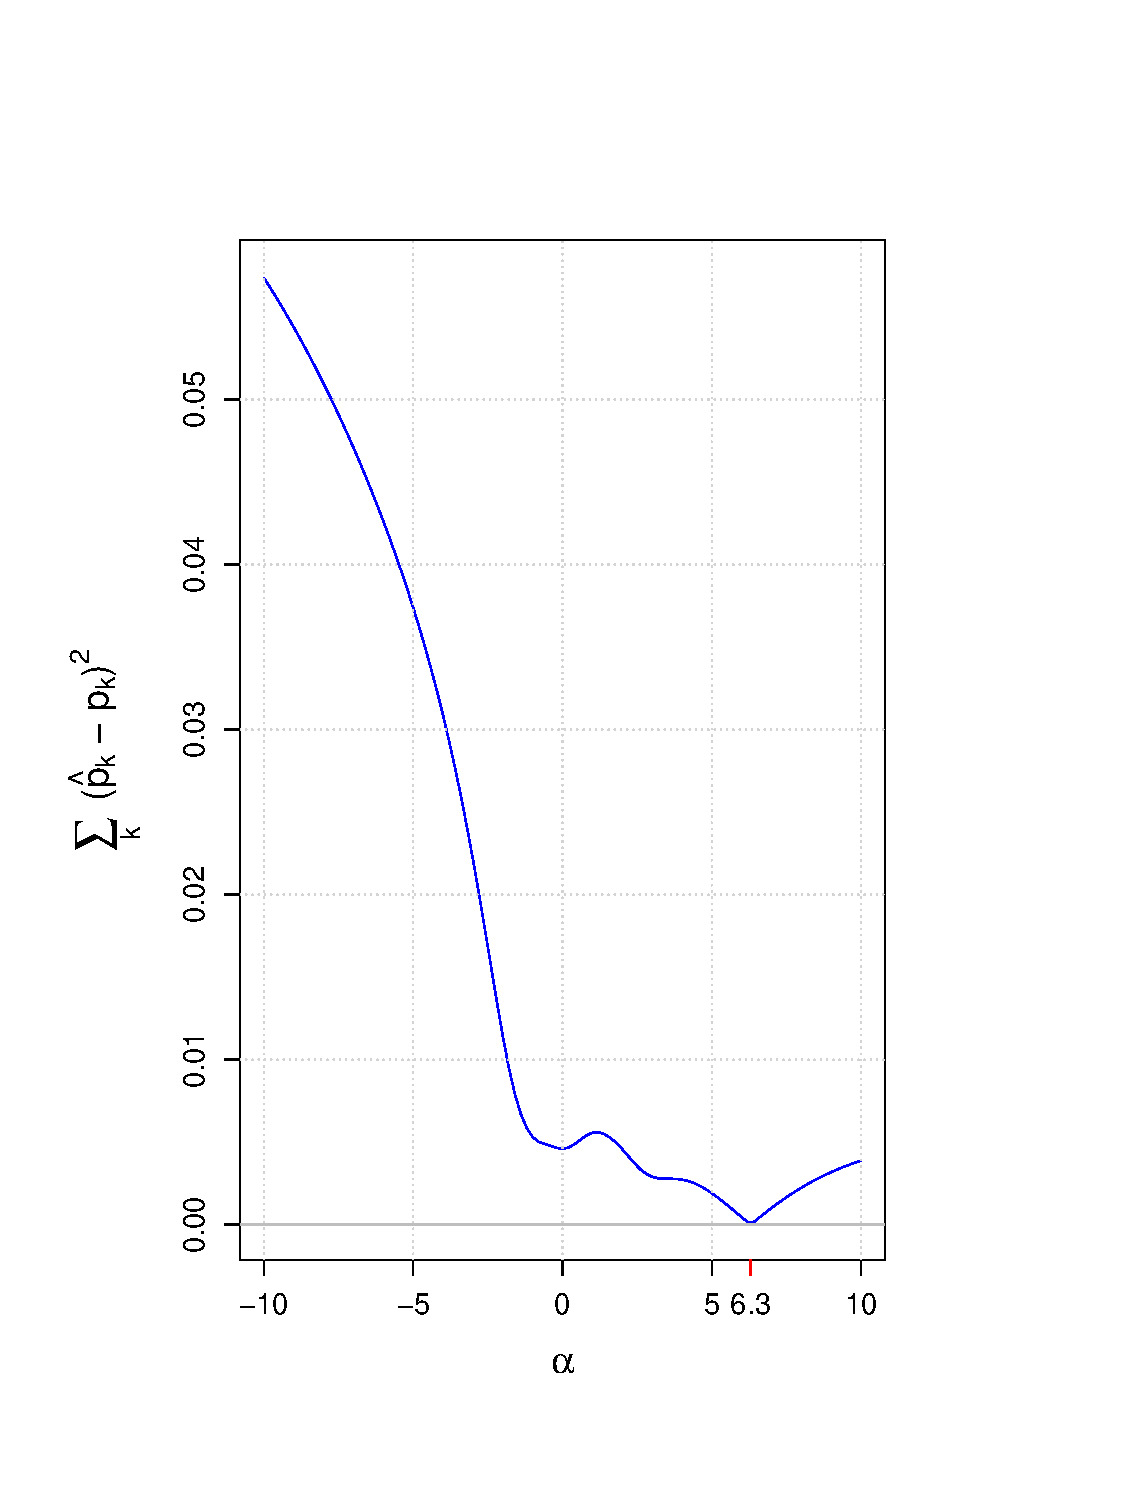
\includegraphics[width=\linewidth]{alpha_trace_6_3.pdf}
  \caption{ $\alpha = 6.3$.}
  \label{fig: alpha_positive}
\end{subfigure}%
\begin{subfigure}{.25\textwidth}
  \centering
  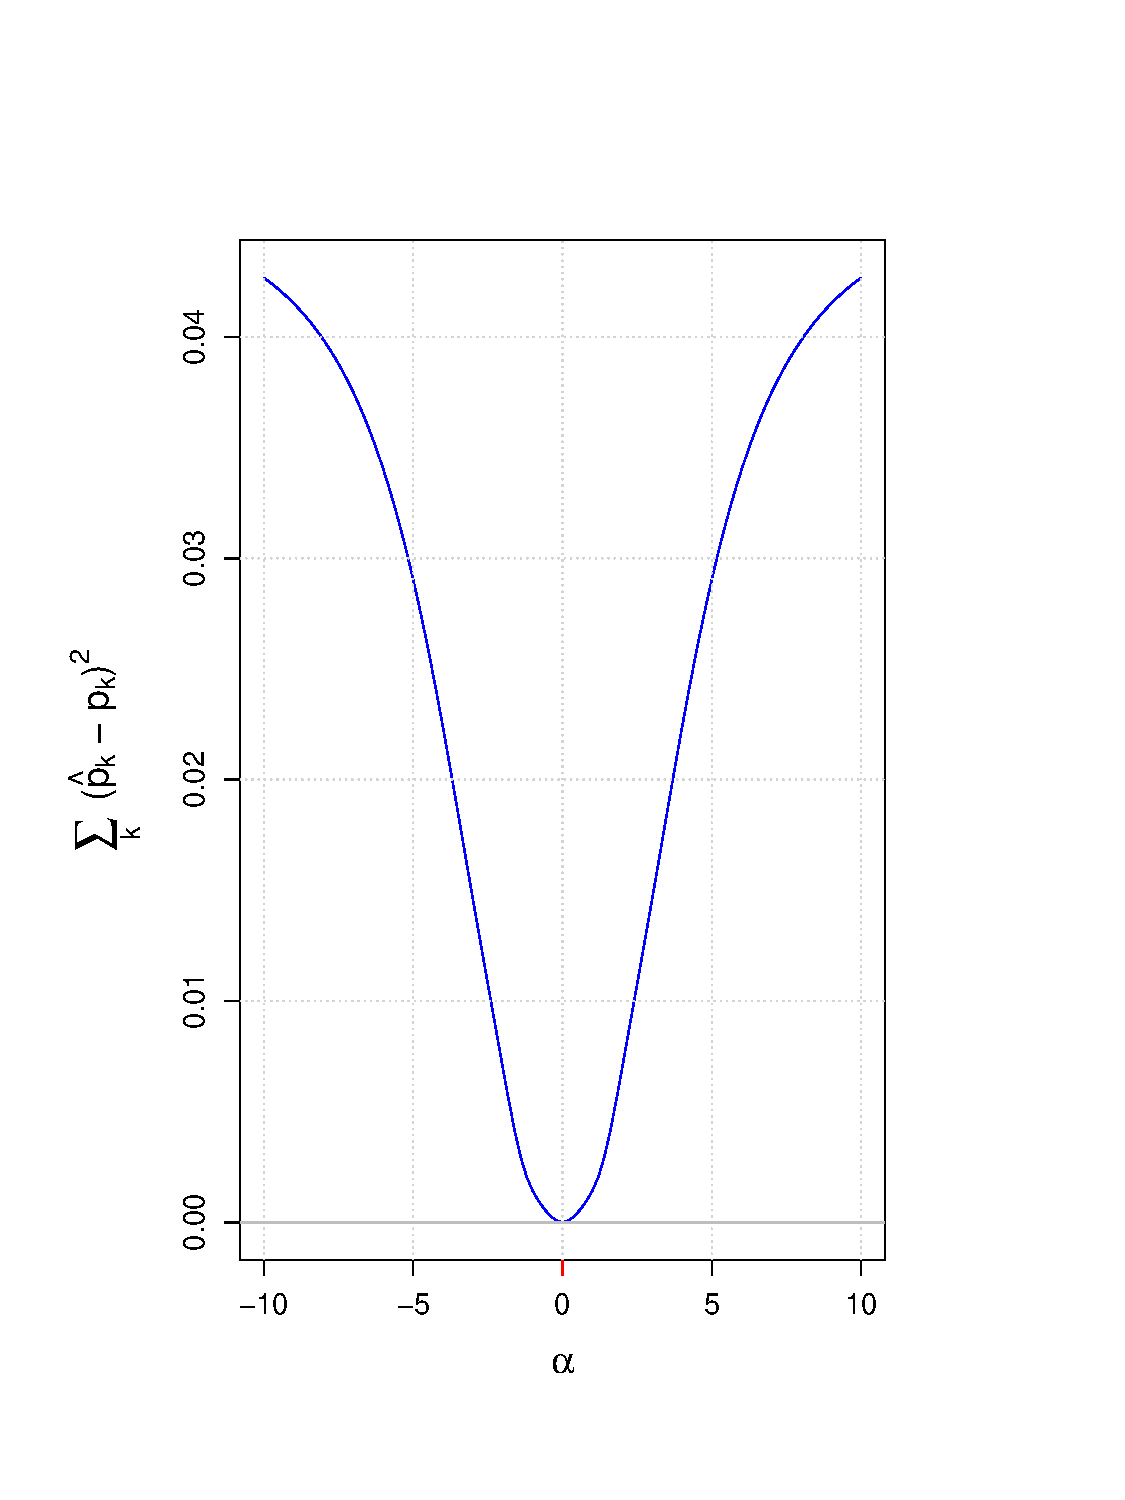
\includegraphics[width=\linewidth]{alpha_trace_0.pdf}
  \caption{ $\alpha = 0$.}
  \label{fig: alpha0}
\end{subfigure}%
\begin{subfigure}{.25\textwidth}
  \centering
  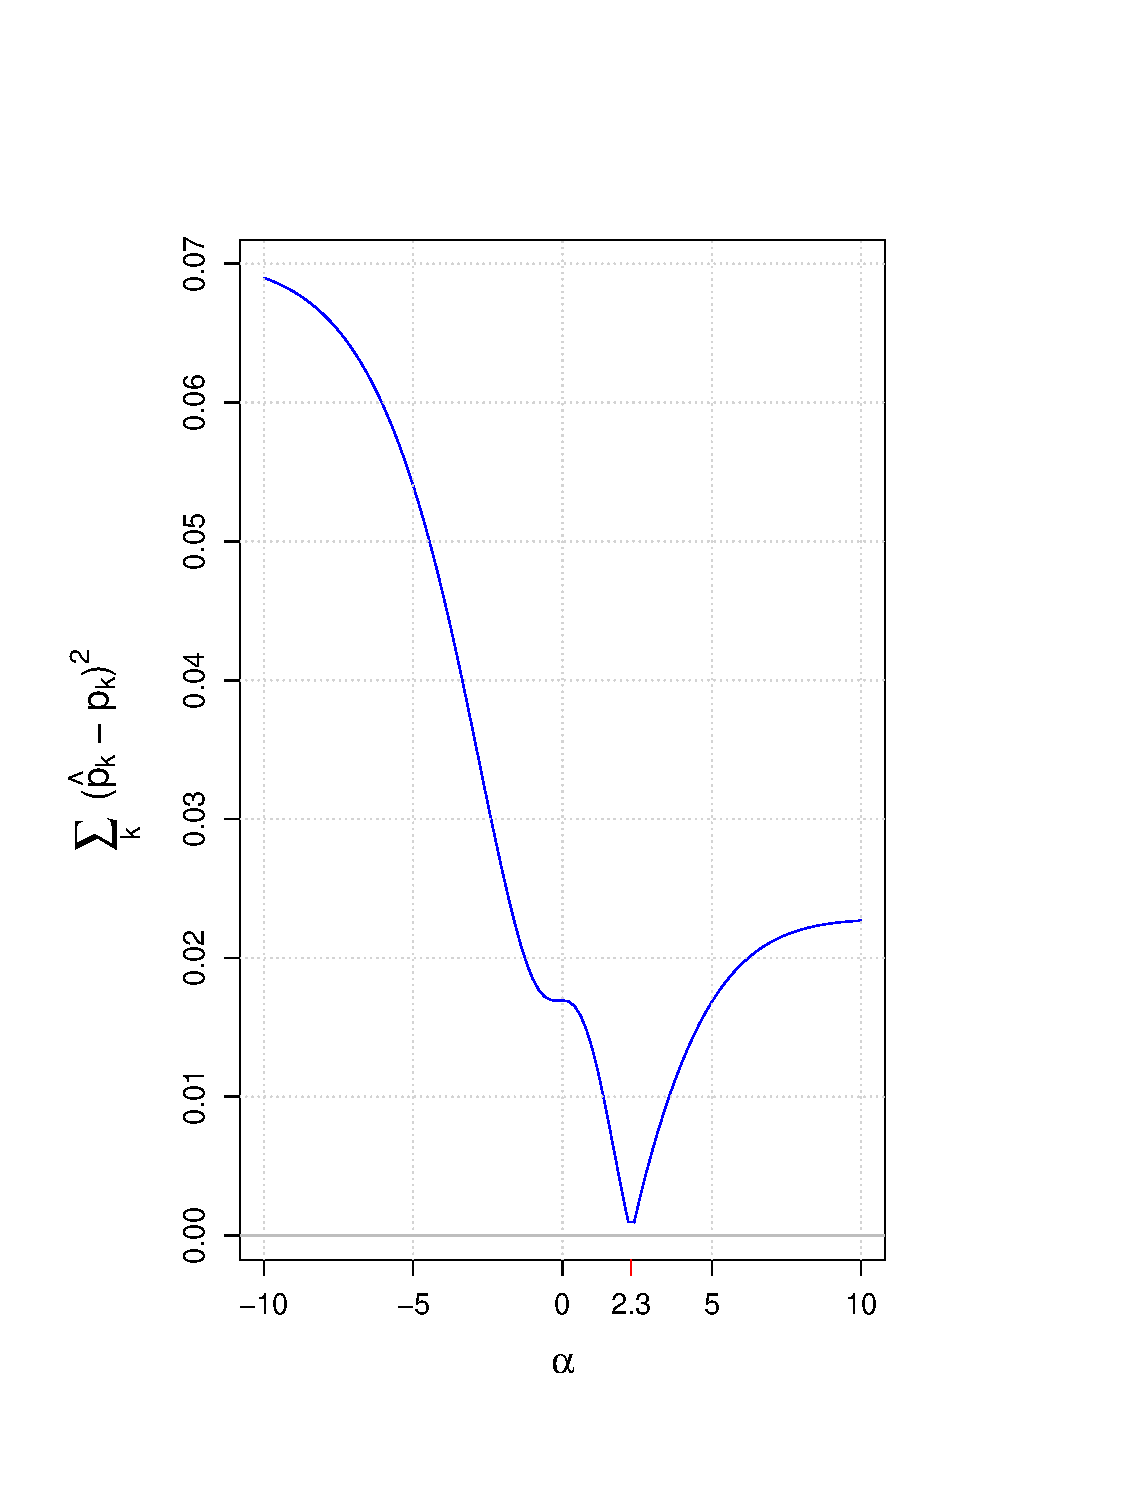
\includegraphics[width=\linewidth]{alpha_trace_2_3_shift_0_2_scale_0_8.pdf}
  \caption{ $\alpha = 2.3$.}
  \label{fig: alpha_shift_and_scale}
\end{subfigure}%
\end{figure}

\end{document}